\documentclass[a4paper,12pt,twoside,openany]{memoir}
\setheadfoot{28pt}{1cm}

%%% DIVERSE PAKKER %%%
\usepackage{float}

% Listings til kode

\usepackage{listings}
\lstloadlanguages{[Sharp]C}
\renewcommand\lstlistingname{Code example}

\lstset{ %
language=[Sharp]C,              % the language of the code
%basicstyle=\footnotesize,      % the size of the fonts that are used for the code
numbers=left,                   % where to put the line-numbers
%numberstyle=\footnotesize,     % the size of the fonts that are used for the line-numbers
stepnumber=1,                   % the step between two line-numbers. If it's 1, each line 
                                % will be numbered
numbersep=5pt,                  % how far the line-numbers are from the code
%backgroundcolor=\color{white}, % choose the background color. You must add \usepackage{color}
showspaces=false,               % show spaces adding particular underscores
showstringspaces=false,         % underline spaces within strings
showtabs=false,                 % show tabs within strings adding particular underscores
frame=single,                   % adds a frame around the code
tabsize=2,                      % sets default tabsize to 2 spaces
captionpos=t,                   % sets the caption-position to top
breaklines=true,                % sets automatic line breaking
breakatwhitespace=false,         % sets if automatic breaks should only happen at whitespace
%title=\lstname,                % show the filename of files included with \lstinputlisting;
                                % also try caption instead of title
%escapeinside={\%*}{*)},        % if you want to add a comment within your code
%morekeywords={*,...}           % if you want to add more keywords to the set
}

% Dansk orddeling
\usepackage[english]{babel}

%Floats og [H]
\usepackage{float}

% Nummering af eksempler og sætninger
\usepackage{amsthm}
\theoremstyle{definition}
\newtheorem{example}{Example}
\newtheorem{theorem}{Theorem}

% Giver mulighed for at bruge æ, ø og å i .tex-filer
\usepackage[utf8x]{inputenc}

% Hjælper med orddeling ved æ, ø og å. Sætter fontene til at
% være ps-fonte, i stedet for bmp
\usepackage[T1]{fontenc}

% Pakke, der gør det muligt at anvende grafikfiler, samt andvende flere captions på samme figure
\usepackage{graphicx}
\usepackage{caption}
\usepackage{subcaption}

% Pakker, der kan udelades, hvis man ikke gør megen brug af matematik
\usepackage{amsmath}
\usepackage{amssymb}

% Pakke, der kan indsætte nødvendige mellemrum efter
% makro-anvendelser.
\usepackage{xspace}

% Retter forskellige bugs i LaTeX-kernen
\usepackage{fixltx2e}

% Indsæt rettelser og lignende med \fixme{...} med "final"
% i stedet for "draft" udløses en error for hver fixme,
% når der compiles.
\usepackage[footnote,draft,english,silent,nomargin]{fixme}

% Gør det muligt at definere farver.
% Se en.wikibooks.org/wiki/LaTeX/Colors for mere info.
\usepackage{color}
\usepackage[usenames,dvipsnames]{xcolor}

%Hyperlinks i indholdsfortegnelse
\usepackage{hyperref}

%Itemization i tables og andet leg
\usepackage{tabularx}
\usepackage{booktabs} % http://ctan.org/pkg/booktabs
\newcommand{\tabitem}{~~\llap{\textbullet}~~}

\hypersetup{
	bookmarks=true,  % Vis 'bookmark'-ramme.
	colorlinks=true, % True = links har farver, False = links har rammer
	citecolor=black,  % Linkfarve for referencer.
	linkcolor=black,  % Linkfarve i indholdsfortegnelse
	urlcolor=black,   % Linkfarve for eksterne URL'er.
}

%%% LITTERATURLISTE %%%
\usepackage[square,numbers]{natbib}
\usepackage{url}

%%% MARGINER %%%
\setlrmarginsandblock{3.5cm}{2.5cm}{*}	% \setlrmarginsandblock{Indbinding}{Kant}{Ratio}
\setulmarginsandblock{2.5cm}{3.0cm}{*}	% \setulmarginsandblock{Top}{Bund}{Ratio}
\checkandfixthelayout 			% Laver forskellige beregninger og sætter de almindelige længder op til brug ikke memoir pakker


%%% OTHER STUFF %%%
\newcommand{\pdf}{PDF}

\newcommand{\Z}{\ensuremath{\mathbb{Z}}\xspace}

% Kommando, der sikrer ensartede referencer til figurer

\newcommand{\figref}[1]{Figure \ref{#1}}

\newcommand{\mgd}[2]{\ensuremath{\{ #1 \mid #2 \}}}

%\newtheorem{saetning}{S�tning}
\newtheorem{definition}{Definition}




\usepackage{cleveref}
\crefname{listing}{code example}{code examples}
\usepackage{todonotes}

% Valg a kapiteludseende
\definecolor{numbercolor}{gray}{0.7}			% Definerer en farve til brug til kapiteludseende
\newif\ifchapternonum

\makechapterstyle{jenor}{									% Definerer kapiteludseende -->
  \renewcommand\printchaptername{}
  \renewcommand\printchapternum{}
  \renewcommand\printchapternonum{\chapternonumtrue}
  \renewcommand\chaptitlefont{\fontfamily{pbk}\fontseries{db}\fontshape{n}\fontsize{25}{35}\selectfont\raggedleft}
  \renewcommand\chapnumfont{\fontfamily{pbk}\fontseries{m}\fontshape{n}\fontsize{1in}{0in}\selectfont\color{numbercolor}}
  \renewcommand\printchaptertitle[1]{%
    \noindent
    \ifchapternonum
    \begin{tabularx}{\textwidth}{X}
    {\let\\\newline\chaptitlefont ##1\par} 
    \end{tabularx}
    \par\vskip-2.5mm\hrule
    \else
    \begin{tabularx}{\textwidth}{Xl}
    {\parbox[b]{\linewidth}{\chaptitlefont ##1}} & \raisebox{-15pt}{\chapnumfont \thechapter}
    \end{tabularx}
    \par\vskip2mm\hrule
    \fi
  }
}																						% <--

%\chapterstyle{jenor}
\usepackage{calc,color}
\newif\ifNoChapNumber
\newcommand\Vlines{%
\def\VL{\rule[-2cm]{1pt}{5cm}\hspace{1mm}\relax}
\VL\VL\VL\VL\VL\VL\VL}
\makeatletter
\setlength\midchapskip{0pt}
\makechapterstyle{VZ43}{
\renewcommand\chapternamenum{}
\renewcommand\printchaptername{}
\renewcommand\printchapternum{}
\renewcommand\chapnumfont{\Huge\bfseries\centering}
\renewcommand\chaptitlefont{\Huge\bfseries\raggedright}
\renewcommand\printchaptertitle[1]{%
\Vlines\hspace*{-2em}%
\begin{tabular}{@{}p{1cm} p{\textwidth-3cm}}%
\ifNoChapNumber\relax\else%
\colorbox{black}{\color{white}%
\makebox[.8cm]{\chapnumfont\strut \thechapter}}
\fi
& \chaptitlefont ##1
\end{tabular}
\NoChapNumberfalse
}
\renewcommand\printchapternonum{\NoChapNumbertrue}
}
\makeatother
\chapterstyle{VZ43}



\setsecnumdepth{subsection}		 					% Dybden af nummerede overkrifter (part/chapter/section/subsection)
\maxsecnumdepth{subsection}							% Ændring af dokumentklassens grænse for nummereringsdybde
\settocdepth{subsection} 							% Dybden af indholdsfortegnelsen


%%% FORSIDE %%%
%\title{Dette er rapportens titel}
%\author{Forfatter 1 \\ Forfatter 2}
%\date{November 2011}

% Sørger for LaTeX ikke strækker teksten ved at forhindre
% der bliver tilføjet linieskift, hvis siden ikke er
% fyldt helt ud.
\raggedbottom 



\begin{document}

%  A simple AAU report template.
%  2012-04-20 v. 0.2.0
%  Copyright 2010-2012 by Jesper Kjær Nielsen <jkn@es.aau.dk>
%
%  This is free software: you can redistribute it and/or modify
%  it under the terms of the GNU General Public License as published by
%  the Free Software Foundation, either version 3 of the License, or
%  (at your option) any later version.
%
%  This is distributed in the hope that it will be useful,
%  but WITHOUT ANY WARRANTY; without even the implied warranty of
%  MERCHANTABILITY or FITNESS FOR A PARTICULAR PURPOSE.  See the
%  GNU General Public License for more details.
%
%  You can find the GNU General Public License at <http://www.gnu.org/licenses/>.
%
%\pdfbookmark[0]{Front page}{label:frontpage}%
%\begin{titlepage}
	%\addtolength{\hoffset}{0.5\evensidemargin-0.5\oddsidemargin} % set equal margins on the frontpage - remove this line if you want default margins
	\thispagestyle{empty}
%	\ThisTileWallPaper{\paperwidth}{\paperheight}{billeder/aau_cover.png}

	\vspace*{\fill}

	\noindent \colorbox{gray}{
		\parbox{\textwidth}{%
			\color{white}%
			\begin{center}
				\Huge{{\fontfamily{ua1}\selectfont Title}} % insert your title here
			\end{center}
			\begin{center}
			\Large{\textsf{Group sw702e14}}\\
			[0.5cm] % insert your subtitle here
			\small{
			%Names here\\
			}
			\end{center}
		}}
		
	\vfill


	\begin{figure}[htbp]
	\centering
	%\includegraphics[width=90mm]{billeder/...}
	\vspace{140px}
	\end{figure}
	
	\noindent \colorbox{white}{
		\begin{minipage}[b]{6.5cm}
		\begin{center}
		%	\includegraphics[width=150px]{billeder/aau_new_logo}
			\end{center}
			\vspace*{-20px}
			%{\small \textcolor{aaublue}{Department of Computer Science}}  \\
			%{\small \textcolor{aaublue}{Software Engineering}}
		\end{minipage}
	} 
	\hfill  
	\colorbox{white}{ 
		\begin{minipage}[b]{3.5cm}	 
			\flushright
			{\large Fall 2014} \\
		\end{minipage}
	}

%\end{titlepage}
\clearpage

\cleardoublepage

\frontmatter
%\Blankpage
\phantomsection
\thispagestyle{empty}
% Titlepage [START]
    \sectionmark{Titlepage}

    \begin{tabular}{r}
        \parbox{\textwidth}{\raisebox{-15mm}{
\includegraphics[height=3cm]{billeder/aauLogoEnStudent.png}} %
         \hfill \parbox{4.9cm}{ %
            \begin{tabular}{l} 
                {\textsf{\small{\textbf{Department of Computer Science}}}}\\
                {\textsf{\small{\textbf{Software 7th semester}}}}\\
                {\textsf{\small{Address: Selma Lagerlöfs Vej 300}}} \\
                {\textsf{\small{\hspace{14 mm} 9220 Aalborg Øst }}} \\
                {\textsf{\small{Phone no.: 99 40 99 40}}} \\
                {\textsf{\small{Fax no.: 99 40 97 98}}} \\
                {\textsf{\small{Homepage: \url{http://www.cs.aau.dk}}}}
            \end{tabular}}}
    \end{tabular}
    
    \begin{tabular}{cc}
	
        \parbox[3cm]{7cm}{ %
	\vspace{7mm}
            \begin{description}
                \item {\textbf{Project title}:} \\
                    A Multiplayer Game Development Framework
                    \hspace{4cm}
                \item {\textbf{Subject}:} \\
                    Internet Technology
            \end{description}
	\vspace{-4mm}
            \parbox{8cm}{ %
                \begin{description}
                    \item {\textbf{Project periode}:} \\
                        Fall 2014
                    \hspace{4cm}
                    \item {\textbf{Group name}:} \\
                        sw702e14
                    \hspace{4cm}
                    \item {\textbf{Supervisor}:} \\
                        Ivan Aaen
                    \item {\textbf{Group members}:}\\%\newcommand{\sh}{18pt}\\%
                    Casper Holst Laustsen\\[0.20cm]
                    Christoffer Nduru\\[0.20cm]
                    Dan Skøtt Petersen\\[0.20cm]
                    Johan Leth Gregersen\\[0.20cm]
                    Kristian Mikkel Thomsen\\[0.20cm]
                    Morten Møller Jakobsen
                \end{description}
            }
	    \vspace{-4mm}
            \begin{description}
                \item {\textbf{Copies}:} 8
                \item {\textbf{Pages}:} \pageref{LastPage}
                \item {\textbf{Appendices}: 0} 
                \item {\textbf{Finished}: 18/12/2014} 
            \end{description}
            \vfill 
        } &
        \parbox{7cm}{ %
            %\vspace{.15cm} %
            \hfill %
            \begin{tabular}{l}%
                {\textbf{Abstract}:}\bigskip \\%
                \fbox{ %
                    \parbox{6.2cm}{\bigskip %
                    {\vfill{\small %
                     %Purpose: To give readers a quick identification of the basic content of the thesis. It should “stand on its own” and be a self-contained document. There should be no need to look elsewhere in the thesis for an understanding of what is said in the abstract.
%1: Objectives and scope
%2: A description of the methods used
%3: A summary of the results
%4: A statement of the main conclusions
                        \bigskip}}%
                    }}%
            \end{tabular}%
        }
    \end{tabular}

    \noindent{\footnotesize\emph{The material in this report is freely and publicly available, publication with source reference is only allowed with authors' permission.}}
% Titlepage [END]
%\Blankpage

\cleardoublepage


% De vigtigste forskelle mellem \include og \input ligger i at
% \include kun må findes EFTER preamblen og at 
% inkluderede filer kan fravælges ved generering af output
% ved brug sammen med \includeonly.

% Se arbejdsblad-skabelon.tex for et eksempel herpå.

\thispagestyle{empty}
\section*{Preface}
This report was written by six 7th semester software engineering students from Aalborg University.\\

\noindent The report documents the development of a framework for meant for developing location-based multiplayer games.

\noindent The source code for this project including raw test data is accessible through one of the following links:
\begin{itemize}
\item \url{http://goo.gl/MjpyXz}
\item \url{https://www.dropbox.com/s/9y1zmsq3evn5vu5/sw702e14_SOURCE.zip}
\end{itemize}

\vspace{.2cm}
\noindent We would like to thank our supervisor Ivan Aaen for providing guidance and feedback.

\begin{table}[H]
	\centering
	\vspace{2cm}
		\begin{tabular}{c c c}
			\underline{\phantom{JAERJAERJAERJAERGO}} & \phantom{cookies} & \underline{\phantom{JAERJAERJAERJAERGO}} \\
			Casper Holst Laustsen & \phantom{cookies} & Christoffer Ndũrũ\\[1.5cm]
		    \underline{\phantom{JAERJAERJAERJAERGO}} & \phantom{cookies} & \underline{\phantom{JAERJAERJAERJAERGO}} \\
			Dan Skøtt Petersen & \phantom{cookies} & Johan Leth Gregersen\\[1.5cm]
			\underline{\phantom{JAERJAERJAERJAERGO}} & \phantom{cookies} & \underline{\phantom{JAERJAERJAERJAERGO}} \\ 
			Kristian Mikkel Thomsen & \phantom{cookies} & Morten Møller Jakobsen\\[.5cm]				
		\end{tabular}
\end{table}


% For at sikre sideskift efter forord. Denne kommando bør kun bruges i
% absolutte undtagelsestilfælde.

\newpage
\mainmatter
\tableofcontents*
\newpage

% % % % New stuff % % % % % % % 
%Main parts of report
\listoffixmes

%Introduktion
\chapter{Introduction}
\label{chap:intro}
%http://thesistips.wordpress.com/2012/03/25/how-to-write-your-introduction-abstract-and-summary/

% It introduces the problem and motivation for the study.

% - Tell the reader what the topic of the report is.
% - Explain why this topic is important or relevant.

% It provides a brief summary of previous engineering and/or scientific work on the topic.
% - Here you present an overview what is known about the problem.  You would typically cite earlier studies conducted on the same topic and/or at this same site, and in doing so, you should reveal the yawning void in the knowledge that your brilliant research will fill.

% It outlines the purpose and specific objectives of the project.
Development of an online multiplayer game serving many users can be split into two parts: Creating the actual game functionality, and creating the underlying architecture to support it. When developing new games these parts are possibly mixed together as the underlying architecture is only used for the specific game. This has the consequence that the developer possibly writes a game specific architecture, and not a general architecture. In some cases, the developer may want to create other similar games with the same underlying structure, but since the architecture and the game itself are intertwined, it is difficult to reuse the same structure. The developer would have to first search through the previous model and extract the desired features, which costs some time. Furthermore, the functionality might not be an exact match to the needs of the new game, requiring additional time to adjust the code.

The focus of this project is to create a flexible and reliable architecture for a server that supports client based multiplayer games. The goal is to allow easy development of multiplayer games for smartphones, and to make it possible for developers to focus on the game development without having to worry about managing the underlying architecture.

The framework will focus on creating a platform for games centered around the location of the player. It has to be scalable, and therefore the server should easily be able to handle multiple games and multiple devices (players) at the same time. This means it is a requirement that multiple clients should be able to connect to the server and perform different actions at the same time. The framework should be able to handle GPS-coordinates, using it as the base of some sort of action, depending on the game implementation of the game, e.g. in a shooter game you are able to shoot players within a certain distance. 

Creating new games from scratch requires both time and monetary investments. While some companies might have these resources available, it could increase the potential profit if some of these resources could be saved. The extra time either means a bigger profit for the developer or more time to work on game features. We argue that creating a flexible framework could help improve this situation.

A framework serves as a basic set of functionality and structural guidelines for the game to be built upon. Overall, game development rarely fits traditional software development process, such as the waterfall method, as requirements can change quickly, and therefore an agile development process is often used \cite{Gamedevelopment}. This means that functionality might have to change on a frequent basis, and whether this means adding new functionality or rewriting already existing functions, a game with an intertwined framework and game will take more time to rewrite, because components often have or provide dependencies for other parts. Therefore it is important to have a clear seperation of the framework and the game.\\

Consider a third person shooter game where functionality revolves around specific gun types and their properties. Far into the development, another gun type might be a new requirement. The developer would, depending on the existing framework have to rewrite much of the code regarding guns in general to suddenly include new functionality. This requires a lot of extra time compared to having a framework that allows easy addition and removal of gun functionality. It is even worse if you end up having to abandon an idea and create something entirely different. Having to rewrite all the code would be tedious, especially when it involves the framework. Having an independent framework could help alleviate this issue.

The size and the amount of divisions of a developing company also matters. The more different people working on a project, the more precision is needed both in the documentation and the framework. Having multiple people writing code on the same game requires the underlying architecture to be as consistent as possible. Changing something in the framework or the underlying architecture requires a notification to all different divisions and people working on the game and it may result in some code refactoring to accommodate the changes \cite{Gameprod}. According to \citet{Gamedesign}, the big companies often create their own framework and document it through the game design document in order for it to fit exactly their needs. This causes them to have a consistent and steady framework to work on, and work individually without consulting different divisions. Smaller companies may not have the luxury of creating a completely game specific framework for each of their projects resulting in them having to spend more work hours adjusting their code to what their co-developers have coded.

Another problem with developing different games from scratch as opposed to having a standardized framework is compatibility. Having different types of devices with different versions of various operating systems means that some devices might not be compatible with the program. What this means is that programs act differently on different devices. With an existing framework this only has to be implemented once. Having a framework that is already compatible with the different devices allows the developers to focus solely on the game, and therefore limiting the amount of time needed for creating portable code.

Constructing a framework that can be used by different developers could save the developer a lot of time and money if the developer uses the framework as intended. It could and should make it easier for the developer to produce code, giving him less work hours needed to create the same content he otherwise would. The struggle with creating a framework like this is that it has to be flexible enough for game developers to create diverse games, but still be precise enough for the developers to not have to write an a lot of code, in order to fit it to the game.

The goal is widely pursued in the form of game engines and general APIs. A large amount of games being developed, are developed on top of already existing game engines. An example of a game engine is the `Adventure Game Studio', providing an API for creating games in third person perspective along with support for pre-rendering. The developer, Chris Jones, has created different functionality he deemed important for creating these games and published it in the form of a simple IDE for game developers \cite{adv-game}. It is specific in the way it focuses on third person adventure games, includign functionality that is relevant for this type of game.
Another example of game engines, is full blown engines with multiple purposes for a specific genre. One of the most used engines for first person shooters is the "Unreal Engine" which is used for many major shooter or fighter games. It is used both as a visual aid, providing 3D rendering, but also provides pre-rendering functionality.

% It provides a ‘road map’ for the rest of the report.
% - This is so that the reader knows what’s coming and sees the logic of your organization.
% - Describe (in approximately one sentence each) the contents of each of the report/thesis chapters.

\section{Problem Statement}
\label{sec:probstate}
When creating games time and money are valuable resources. To ensure a high amount of quality code, the developer has to spent a lot of time writing code that could be found in a generic framework, increasing the cost unnecessarily. This naturally raises the question:

%\mbox{\parbox[b][2.5cm][c]{0.95\textwidth}{\textit{How can we develop a framework for creating multiplayer games - increasing the experience for the developers.}}}

\mbox{\parbox[b][2.5cm][c]{0.95\textwidth}{\textit{How can a flexible framework for creating multiplayer games be developed?}}}\fxfatal{Bør stadig overvejes!}

\noindent The idea is simple: we want to create a framework for creating simple location-based multiplayer shooter games. In order to properly answer the stated problem, these goals should be fulfilled:

\paragraph{Flexibility} The framework has to be as flexible as possible. I.e., it should allow implementation of as broad a spectrum of games as possible within the mentioned genre.
\paragraph{Scalability} The framework should be able to handle multiple games, each with multiple users. The purpose of hosting several games at once is to allow development of relatively short games with a limited number of players each, e.g. a group of friends.
\paragraph{Ease of Use} The framework has to be easy to use for developers. If it is too complicated it will not be as attractive to start using - the idea is to make development easier rather than harder.





%Scenarios
%\section{Scenario 1: Maps \& Navigation - City Areas}
In a large city, for example one of the 5 largest cities in Denmark, data connectivity can be obscured by many big buildings, concrete parking garages or when entering the the subway. This type of data connection loss can be unpredictable and happen in an instant, but it can be expected to be relatively short. 

A scenario can be a travelling salesman arriving at an unknown large city. The salesman is trying to find a customer and have to navigate through public transportation. The customer is awaiting the salesman for a business meeting, and therefore the salesman is limited by time. The salesman is relying on information about public transport timetables and a journey planner to direct him to the customer. 

A number of challenges may arise for the salesman regarding connectivity issues. The salesman may have plans to ride one bus to the customer, but upon arriving at the bus stop he realises the bus is delayed. He now has to consult his device for an alternative bus to ride. Since the salesman is under time pressure, he is relying heavily on having data-connection. Another challenge may arise if the salesman descents into the metro-station. The salesman may have become confused about which train to enter, and is now relying on still having a data connection. The subway is underground and built from concrete, which may severely reduce the strength of the data connection. 

The challenges arise when the salesman is under time pressure and has to deal with unpredictable traffic and public transportation. The salesman would be more secure if a service would be able to provide the desired information even if the device has lost data-connection.
%\section{Scenario 2: Maps \& Navigation - Countryside Areas}
When travelling out of cities, data connectivity can be unavailable for a longer period of time. This type of data connection loss is slowly fading away as you move further away from the connection source.

A scenario can be a couple going for a walk in the woods on the countryside. They are visiting an unknown area and walks into the woods. They happen to get lost and wants to find their way back to the car, but in the woods no data connection is available and they are lost.

A modification of this scenario could be a couple that wants to get additional knowledge of the area they are walking around in, e.g. visiting Rold skov in Denmark, they might want to read the stories about the robbers from Rold. It is also possible that they want to know about the attractions in the area, and directions to them.

The challenges are predicting that the data connection will be lost in the near future, and what services should be attempted to download to a mobile device. 

%\section{Scenario 3: Bus and Train}
In this scenario the problem be solved is to minimize Internet drop-outs when travelling on frequently used bus or train lines. The idea is to collect data on a user base and use that data to identify areas where the user might lose connection.

The solution should be able to detect travelling by bus or train and predict the route and destination. It should reduce the user experience of no Internet during the travel and make relevant information available for the destination, should it be in a poorly connected area.



%In order to do so several approaches are available.

%A simple approach is to measure the signal strength of the device and use that as the base for predicting when connection will be unavailable. Using this method a stable but slowly dropping signal strength might indicate a future with no connection available, in this event the required web resources should be cached so they are available doing an offline period. Another scenario could when the signal is unstable but the average remains high, this could indicate interference in the area but no risk of a significant offline period, in this case caching is not necessary.
%
%Another approach is to base the prediction on historical data of the near area. This can be done by gathering data of where Internet connections usually drops and build a map for the available providers. Then the caching will be done when a device is predicted to move into such an area.

%Problem statement
% How can a user be guaranteed to always have relevant information available, regardless of network connectivity?
\section{Chapter Descriptions}
The following is a brief description of each chapter in the report

% add more here as report progresses %
\paragraph{From Idea to Framework}
This chapter will give a general idea behind the choices made - why we chose to make a game and what outcome expect to get from it. It will give a short description of the overlying architecture and goal of the framework. 
\paragraph{The Game}
This chapter will describe the game we used a foundation for creating a framework. It will describe the client, how it was designed and lastly how it was implemented.
\paragraph{The Framework}
This chapter describes all of the choices considered for the framework. It will describe how the game influenced the server and framework and advantages and disadvantages of this. Furthermore it will describe design and implementation of the server and database. Lastly a section will describe tests and the result of it.
\paragraph{Conclusion}
A brief summary of the entirety of the project and an evaluation of whether the project upholds the goals of the project.



%From Idea to Framework
\chapter{From Idea to Framework}

This chapter describes the general methodology behind the entire project. It will describe the underlying architecture. It will furthermore describe how and why we have taken the approach we have, and describe advantages and disadvantages to it.

We have chosen to develop the framework simultaneously with a game based on the functionality provided by it. The idea behind this work method is to ensure the framework entails all the requirements needed to create a game. Furthermore it was developed to validate the framework is good enough to create a detailed game without being specifically programmed for it.

\section{Architecture of the Project}
%
% A description of the entire architecture. server, client and which part takes care of what (initially and optimally).
%

% intro
The project as physical entities, is separated into two parts. A server and a client part.\\

% client
The client (the player) does not perform any computation. Instead it generates information meaningful to the server based on what the player does, which is then sent to the server. The player could for example shoot someone in the game, and would then send data to the server requesting it to record this action. \\

% server
The server receives data from the client which describes what has happened on the client-side. The server then determines the correct action to perform. This could be logging the client in after receiving a login request from the client in the data, or the client wishing to join a game.\\

% reasoning
The reasons for separating the project into server and player entities are multiple. One is that it would be power consuming for a player, playing a game on a mobile device developed with the framework, to host a game for their friends. The mobile phone would have to perform all computations for the game they are playing and host the database. When a single central server is used for these computations, the server can be located at some location and be plugged into the power grid, thus averting the power supply issue. Also, the players woud have to know the address of the device hosting the game to join, unless some mechanism was devised to handle this.\\

Another advantage to splitting the project up in two parts, instead of creating it as one application, is portability. Since the client itself is thin, because the heavy operations are performed on the server, it requires less work to port the client to other platforms. Less code and complexity on the client-side equals less work to rewrite the client-side if porting the client to a different platform.
\section{Frameworks}

In the context of software, a framework is a solution which provides a set of functionality much like a library, but with small differences. It provides functionality for development of products, either independently or as part of a larger platform.
Generally the flow of control is dictated by the framework rather than the user. The framework often have a default behavior, in case an important functionality is not overridden by the user. The most important detail is however that the framework code should never be modifiable by the user - the user should rather build upon the framework. \cite{framework}

A framework can include other smaller parts such as other programs, tools, APIs or other libraries. A framework can be confused with an API or a library. A framework is a group of classes, interfaces and other pre-compiled code, while APIs are the public front of a framework, and libraries are specifically made for a single purpose. A well-made framework hides most of the code in assemblies and DLL-files and only shows the above mentioned classes and interfaces. An example of a framework for an online store could be responsible for handling the general flow. In this case it would be handling tasks such as `purchase item', `checkout' or `browse warehouse'.

APIs are made for interaction between applications and with a specific purpose e.g. Google Maps API\cite{google-maps-api}. Google Maps is built with an underlying predefined set of functions, and the API is the manual the developer can use to work with Maps. It can be described as the information necessary to use the provided classes and sets of classes.

A library can be described as a very specific framework. It is a collection of implementations with a well-defined interface - a strict set of functions for a specific purpose. An example could be the timer library in C\#\cite{net-timer}, which provides a simple timer class with a lot of different properties, methods and events.

As we do not have an existing framework to build an API for, we need to create the underlying functionality. This means we have to create either a framework or a library, but seeing we have to create wide spectrum of functionality, the optimal solution would be to create a framework. We can then move on to build an API on top of this.
\section{Seperation of Framework and Game}
%It should be possbile to build a new game on the same framework.
The framework and the game is split into two completely seperate components. This enables creation of a new game on the same framework. 
%Why is the framework and game seperated?
The reason for this choice, is that the framework can be reused for different games. Because of this future developers who would like to make a game can reuse the framework and do not have to touch any framework code, only the game code itself. 
%Why is it a good idea, and what are the tradeoffs?
Developing the framework and game as two completely independent components has a number of good side effects. First of all, it makes it easier to avoid writing code which is intertwined (between the framework and the game). 
%What would happen if it is not split up?
If this was not avoided, it would be very hard to create an independent framework, since part og the game which was developed on top of the framework would be tied into the framework and vice versa. Therefore, a clear code-wise distinction between framework and server produces cleaner, more independent overall program structure. 
%Discuss the constraints of the framework (e.g. database schema, efficiency).
Because the framework and game are separated components, the framework has some limitations. The framework essentially enables development of many kinds of networked multiplayer games. Therefore, the database's tables for example have to be quite ``fixed'', since the developers of the games for the framework should not need to change the database and framework code. A database change will likely warrant some code in the framework to be rewritten. If the developers have to start rewriting code in the framework to develop their game, the point of the framework is lost. 
\section{Model View Controller}
%Describe why an architectural pattern is important

%We chose MVC - describe it

%What do we gain from MVC? What are the tradeoffs?

%Other options? Model-View-Presenter, Observer, Multitier architecture?

%Is it possible to change the architecture?
\section{Interfaces}
%INTRO:
%Server and client both consist of several small parts that all need to communicate.
%Examples: user->client, client->server, game->db...

We have decided that all information between the server and the client are shared in the form of XML. We have chosen to do so because of the diversity XML provides, and its interoperability with a wide variety of software. This fits well within the theme of creating a very customizable framework for creating games. Furthermore we feel that XML is somewhat of a standard for sharing - and many people already know how to make use of it.

\subsection{Client and Server correspondence}

The idea behind the XML output is to create tags for each different kind of data. We have different kinds of data to sent depending on which activity we take on the client side. An example of this could be the login activity on the client side, this requires sending some username and a password for confirmation on the server side.

We create individual methods for each different scenario rather than creating a generic XML converter because we want to enforce the right data structures and types. The example below is the said convert to XML login method. 

\begin{lstlisting}
    public static String login(String username, String password) {

        String tag = "Login";
        String entryA = "Username";
        String entryB = "Password";

        String xml = "";

        xml += "<" + tag + ">";
        xml += "<" + entryA + ">" + username + "</" + entryA + ">";
        xml += "<" + entryB + ">" + password + "</" + entryB + ">";
        xml += "</" + tag + ">";

        return xml;
    }
\end{lstlisting}

It simply converts the input of the variables username and password into XML on the form (except it being on a single string). The information is structured around what the server needs for authentication - so what the client sends is of course built around what the server requires.

\begin{lstlsting}
<Login>
   <Username> USERNAME </Username>
   <Password> PASSWORD </Password>
</Login>
\end{lstlisting}

A basic principle of TCP is that the client always require a response from server before it can move on. For the same reasons mentioned above and for the sake of consistency the client expects XML on roughly the same form. For this example we require an ID for the specific user to load his specific settings/information. We also require a boolean in the case that it wasn't a valid login, this is then handled on the client side. The following code is what a client expects to receive.

\begin{lstlisting}
<Login>
   <Id> IDENTIFICATION </Id>
   <Valid> BOOL </Valid>
</Login>
\end{lstlisting}

XML provides a really easy way to dispatch or deserialize the input - making it an optimal solution for small constant interactions like the ones we need. There are many different alternatives to XML, but we feel that it is a simple interaction without extraordinarily complicated needs - which makes the simplicity of XML a great trait for us.

%PROJECT IMPACT:
%Several sub-groups are developing the different parts, so...
%How does this need for communication impact development?

%We chose to do *like this* - why did we choose that, and was it a good choice, or would something else have been better?

%SOLUTION
%How is this communication done? (How are the interfaces made, and how was it decided?)

%Why is it done like this? Is it efficient? Easy? Scalable? Maintainable? Something else?

%Are there any alternatives? Why not one of them?

%The game
\chapter{The Game}

\section{Game scenario}\label{sec:game}

This section describes the game we have decided to focus on. This game will be implemented as a prototype for proof of concept. It implements different uses of the server functionality that we want to display. It was also created for the purpose of setting a limitation for the server functionality. Otherwise we could have kept creating functionality for multiple different purposes. The game we have decided to create a scenario for, is a game based on the real-life coordinates of the participants. The game should be playable among friends, and be interactive. The game is a prototype that could be implemented on top of our server and item balance, e.g. a certain weapon may be stronger than intended, is in no way to be considered final in the game.

The biggest advantage of creating a specific game scenario is a better insight into the general functionality needed on the server side. It furthermore provides a goal which helps with motivation and work culture, in the sense that we could more easily divide the work needed in the project. One of the drawbacks of using a scenario in this way is that, if one is not not careful, it could cause us to accidentally focus strictly on the scenario, and might exclude functionality that could be useful on the server side. Just because the functionality does not fit a certain scenario does not mean it is not useful for a general model. Furthermore, we might not get the flexibility we look for in a server as we don't have different types of games to test it with.

\subsection{Game Rules}\label{subsec:game-rules}

The following is a description of the game scenario.

\paragraph{Game winning criteria}
The idea is for one of the competing teams to obtain an ultimate relic. Once a team locates it, the game should end with a victory for the team with the relic. At the start of the game it is impossible to know where the relic is located, and you gradually locate it by finding clues around the map.
Another way to win is to be the team with the largest amount of points if a time limit is set and reached.

\paragraph{Objectives}
There is a list of different objectives each with a unique functionality and meaning to the game.
\begin{itemize}
\item Point Objectives - Gives +1 team point, takes 30 seconds to capture and reveals your locations to nearby enemies for 120 seconds.
\item Puzzle Objectives - Gives your team a clue, takes 300 seconds to capture and reveals your location for 600 seconds.
\item Crates - Can contain weapons, instantly acquired and reveals your location for 120 seconds.
\item Powerups - Can contain bonus for your stats,  instantly acquired and reveals your location for 120 seconds.
\item Shrines - Will give different bonuses depending on the shrine type, the shrine is active for 4 hours after activation, takes 300 seconds to capture and reveals your location for 600 seconds.
\item Ultimate relic - Digging for the ultimate relic has a one hour cooldown, takes 300 seconds to capture and reveals your location for 600 seconds.
\item Watchtowers - Gives increased range when within the tower.
\end{itemize}

\paragraph{Items}
There is a list of different items in the game as well. These items are obtainable through crates dropping.
\begin{itemize}
\item Start-pistol - Range: 25 meter, Damage: 20 HP, reveal-time: 60 seconds and cooldown: 20 seconds.
\item Shotgun - Range: 15 meter, Damage: 60 HP, reveal-time: 90 seconds and cooldown: 30 seconds.
\item Sniper - Range: 40-80 meter, Damage: 70 HP, reveal-time: 90 seconds and cooldown: 120 seconds.
\item Ammunition - Pistol ammunition +16 bullets, Shotgun ammunition +4 shells and Sniper Ammunition +3 bullets.
\item Medkit - gives +25 health points on pick up.
\end{itemize}

\paragraph{Powerups}
This is the list of what is obtainable as powerups.
\begin{itemize}
\item Armor - +15 Armor (Max 50 Armor)
\item Vision - +2 meter (Max 50 Meter)
\item Scan - +20 meter (Max 60 Meter)
\item Range - +2\% range (Max 6\% Range)
\item Shield - Blocks the next shot
\end{itemize}

\paragraph{Shrines}
The following is a list of the different shrines and functionality. Shrines expire after a given amount of hours.
\begin{itemize}
\item Power Plant - Provides 2 points every half an hour.
\item Locater - Pinpoints the location of an object in range of scan every half an hour.
\item Shield Generator - Gives the entire team a shield every hour.
\item Factory - Provides each user on the team with 3 pistol bullets, 2 shotgun shells and 1 sniper bullet every half an hour.
\end{itemize}


\section{Client Design}
\section{Client Implementation}
In this section, the implementation of the Client-side of the project is described. The section contains implementation details about the components in the Client, such as the component that handles GPS locations.\\

The implementation is based on the choices and thoughts about the client from the client design in \cref{sec:desClient}
\subsection{Components in the application}
Activities, adapters, interface, GPS etc

%The framework
\chapter{The Framework}

This chapter describes all of the choices considered for the framework. It will describe how the game influenced the server and framework and advantages and disadvantages of this. The chapter focuses on the separation of the framework and the game - it will describe the relationship between different game functions and their framework counterpart. It will describe the implementation of the said features and the possible uses of it. In the end, the test and the result of it will be described.

\subsection{Server Architecture}
\label{sec:server}

The server is structured in three layers: a dispatcher service, a logic layer and a data layer. Because we wanted to develop a framework for creating future location-based games, we had to make a decision how to achieve this goal. We could not interleave framework-specific functionality with the specific game we developed along side our framework. The result was these three layers. We wanted to build a communication layer to handle the interface between the client and the server and a data layer to handle the interface between the server and the database. These two layers were chosen rather intuitively early in the design process. Our next choice was how to choose a way to implement a specific game capable of using the framework, while still being scalable and encapsulated. We decided to make the threaded class called Game Thread handle all game-specific calculations, logics and responses. 
It was helpful to build a game alongside the framework, this helped us to figure out the need for a service to handle timed events in the framework, which resulted in the Event Timer. We also discovered the need for unit to handle client requests that requested functionality prior to the Game Thread. This was requests like logging in, and seeing all active games, which cannot be handled by a game thread yet since it might not be created yet. The result was the Admin. The Event Timer and the Admin are both positioned in the Logic Layer, because they help make logical decisions based on requests made by the client. 

%Server Architecture
\paragraph{Dispatcher Service}
The dispatcher is a service responsible for handling the communication with the client. It consists of an asynchronous I/O\fixme{IO or I/O throughout report?} and the dispatcher itself. Communication is done by an XML interface where requests from the client is verified by the dispatcher and passed to either the Admin module or a Game Thread depending on the message. 

\paragraph{Logic Layer}
This layer represents the business logic of the server application. The Admin module handles user creation, user login and game creation and is general for all game implementations. Game Thread is where specific game logic is implemented and its implementation will vary depending on the type of game. Event Timer is a general module handling events specified to happen at certain times. The game threads are responsible for creating events for themselves. The event timer will then notify a game thread at the specified time. As illustrated in \cref{fig:serverarch}, game threads are not a part of the framework, but can be ``plugged in''\fixme{change word??} to the framework. This increases the versatility of the game threads, since a developer can create his own game threads and plug them into the framework.

\paragraph{Data Layer}
Is the database representation in the model using the data mapper pattern\fxwarning{WE book ref}. The gateway is responsible for querying and updating the database and mapping the tables to objects used in the game logic and administration.

\begin{figure}[H]
  \centering
  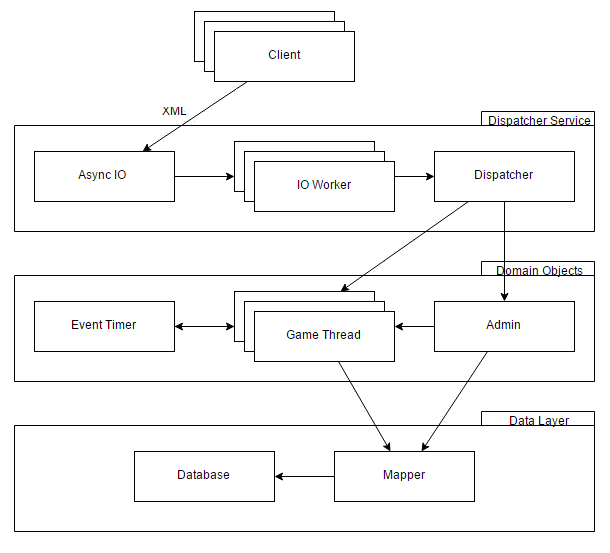
\includegraphics[width=\textwidth]{billeder/serverarch.png}  
  \caption{Architecture of server displaying the branching of an incoming connection}
  \label{fig:serverarch}
\end{figure}

%Dispatcher Service
\subsection{Dispatcher Service}
This layer is responsible for communication with the between client and server, this responsibility is divided between an IO module and a Dispatcher. In this section we will first examine Synchronous and Asynchronous IO in order to determine which is best suited for this framework and then the Dispatcher which forwards messages to the Logic Layer. We decided on Asynchronous IO and base our design on \cite{?} 	 %http://msdn.microsoft.com/en-us/library/fx6588te%28v=vs.110%29.aspx

The Asynchronous IO unit is handling socket creation and TCP/IP communication, a rather trivial part of a client-server interface when you disregard the communication type. The need for out Dispatcher unit has been revealed by building our game. We need a way to dispatch requests from the client to the right component and method on the server. We dispatch to either Admin or Game Thread, by reading the request from the client and determine what type of request it is and continue accordingly. We decided to build the Dispatcher to encapsulate reading and analysing the requests from the client. Alternatively, we could have handed everything to Admin and incorporated the Dispatcher's functionality into the Admin, but we did not consider this a well structured framework.

% ms-syn-asyn - http://msdn.microsoft.com/en-us/library/windows/desktop/aa365683(v=vs.85).aspx


\section{Synchronous vs. Asynchronous I/O}
%What is B/NB I/O?
I/O can be handled either synchronously or asynchronously. A synchronous I/O operation is blocking, i.e., the thread that executes the current job is in a waiting state, where it does not compute anything, until it gets a response. An asynchronous I/O operation is non-blocking and therefore allows the thread to execute another job while waiting for the I/O operation to finish. This is illustrated on \Cref{fig:syncasync}. The figure does not show the overhead caused by using asynchronous I/O, which causes this to not always be the best solution, especially if there are many short I/O operations \cite{ms-syn-asyn}.

\begin{figure}[H]
  \centering
  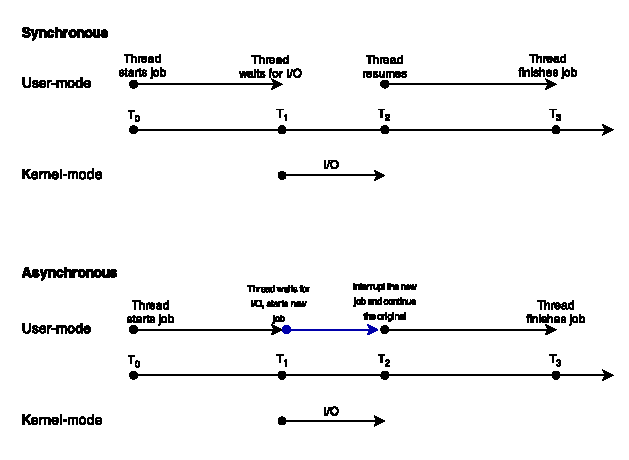
\includegraphics[scale=1.2]{billeder/sync-async.pdf}  
  \caption{Synchronous and asyncronous execution. Based on \cite{ms-syn-asyn}.}
  \label{fig:syncasync}
\end{figure}

This is the case for one or few users, but if there are many users at once they either have to wait in queue for previous I/O operations to finish, or each operation has to be executed in it's own thread, which would potentially result in many active threads, requiring a lot of memory. As pointed out by \citet{amir} it is worth noting that an asynchronous call that results in a synchronous operation causes the application to block, and therefore should be considered during implementation.

To enable the server to scale better, the I/O is implemented asynchronously. When the server receives an input, it is asynchronously sent to a dispatcher which sends it to the correct place; this is described in \Cref{sec:server}. Because of the many parts that have to interact, it is hard to determine if this implementation behaves as expected without testing it, but changing to a synchronous implementation would not be very expensive, as the asynchronous code is very similar to the synchronous code thanks to .NET's \texttt{Async} and \texttt{Await} keywords \cite{ms-asyn}. Making both implementations available at the same time, and letting the user choose which one to use, would also be relatively easy to do, but it adds some extra complexity to the code, as changes in one implementation would require similar changes in the other.
%What are the advantages and disadvantages?

%Which alternative(s) is/are there?

%Why did we make the choice we did?

%How flexible is it?
% - Could it easily be changed? 
% - Could both be implemented and the framework-user decides which one to use?
%
%\section{Synchronous vs. Asynchronous I/O}\fxfatal{This section will be rewritten with proper sources.}
%For the client/server socket communication, a choice between synchronous and asynchronous I/O has to be taken.
%% % blocking % %
%Synchronous I/O can have a better performance than asynchronous, but can cause problems when using a threaded architecture that spawns a new thread for each client. This is particularly true when the server should be scalable in regards to its number of connected clients. There might be 5 and there might be 5000 or even more.
%Tests show that threads are very efficient when it comes to memory and context switching, but only when the threads are kept alive for the entire execution of an application. This is not the case for our application, which will likely have many connections of varying durations during its up-time. \fixme{cite}\\\\
%% % non-blocking % %
%Asynchronous I/O is chosen for this project. It scales well when there are many clients, and the system should scale well with a potentially large number of clients. A notable advantage of asynchronous is that it limits the number of concurrent threads. The server asynchronously accepts a connection request from a client, and then starts an asynchronous worker thread to handle communication with the client. Meanwhile it continues to listen for new client connections.
%

%The ability to scale well does not come for free, however. Non-blocking IO is not always as fast as blocking IO and this can result in decreased performance. 
\subsection{Dispatcher}\label{subsec:dispatcherdesign}
The Dispatcher is a central component in the framework. It is placed in the \textit{Dispatcher Service} in the architecture, and is the first receiving to interpret a request sent by a client. The dispatcher simply dispatches a call to the appropriate method with the appropriate parameters when it receives XML data. In order to do this, it reads as little XML as possible to extract information to decide the appropriate destination and the right method to call. It attaches the entire XML as parameter to the method call.

The Dispatcher looks for the specified method call in the XML to hand it over to the Admin class. This is static calling of methods with attached XML. The Dispatcher waits for the Admin to return an XML, which it returns to the Async IO.

The Dispatcher handles all requests to a game thread dynamically, as it only interpret the method call before handing it over to the game thread. It then waits until the game thread returns a XML string, which it returns to the Async IO.

%Logic Layer
\subsection{Logic Layer}
This layer parses and reacts to the messages received from the Dispatcher. The logic layer interact with the Game Threads and consists of the Event Timer module which is callable from the Game Threads and can do a callback at a later time. The layer also contains the Admin module responsible for creating Game threads as well as non-game specifics such as authenticating logins.

The framework allows the user to use services like logging a client in through an XML-based interface. Services in the framework requires the user to implement proper XML-based communication on the client-side. A discussion about the use of XML seen in \fixme{ref til johans afsnit om valg af XML}. The framework also offers to handle Game Events, timed to occur after a specified time-stamp. This service used by creating a Game Event in the Game Thread being build by the user of the framework. We decided to build the Event Timer this way to encapsulate time-handling, and make a generic module that can be used for many different events. The user of the framework can specify what should happen for a given event in the Game Event class.

\subsubsection{Admin}\label{subsec:admindesign}
The Admin module is responsible for handling server-requests not related to specifict Game Threads. The Admin module handles administrative calls like creating new games or accounts as well as verifying login requests. 

%impl?
%A \textit{CreateGame} call cannot be send to a game thread, obviously because the game thread has not yet been created. Therefore this method will create a game from a model-class \textit{Game}, store it in the database with the provided settings, start a thread on the server for it to run on. 


\subsection{Event Timer}\label{subsec:eventtimerdesign}


%Game Block
\subsection{Game Block}
This is the workstation of the user of the framework. This block interacts with all the layers in the framework and makes use of the functionality provided by the framework. This class encapsulates all game-specific logic.

This is where we designed the framework to allow the user to develop a game. The framework has several rules the user has to follow when using the framework. They are explained for each module in the design. An example is the XML communication from client to server.
 
\subsection{Game thread-pool}
The game thread-pool is a collection of active game thread-instances, uniquely identified by a game-Id.

The game thread-pool is used as a handle to the game threads, and allows dynamic call to the desired game through method-parametrization. 

\subsection{Game thread}
\paragraph{Starting a game}
A game thread will be initialised and started when a user requests to host a game. A game will be assigned a game-id by the server, user-specified settings for hosting the game will be initialised and the game will be created in the database. 

When the server initialises each setting, it calls a method within the game thread-class. These methods calls the database-controller to change the state of the game in the database. These settings are:
\begin{itemize}
\item Game-privacy (Public or private game)
\item Number of teams
\item Game start-time
\item Game end-time
\item Game-boundary NorthWest GPS-coordinate
\item Game-boundary SouthEast GPS-coordinate
\end{itemize}

\paragraph{Updating a game}
Updates to a game can be split into two groups. One group is specific changes to a game, like inviting a new player or firing a gun. Another group is updating a players position when moving around in the game.

Updating a players position is trivial. The game thread receives a game-id, player-id and a new position. It calls the database-controller to store the new position in the database.

When performing an action like firing a gun, the server will have to fetch the gunman's position and the victim's position. It will then calculate if the range of the fired weapon allows the victim to be hit. If the shot is successful it will return that to the player, if the shot is unsuccessful it will return that the victim is out of range. 

All updates to change the state of a game will be in the game thread-class. This class will need to contain methods for all the in-game functionality. 

\paragraph{Closing a game}
When a game ends, the call will come from the timer thread. This will ask the game thread to clean up what is has stored in the database, and return a status message. The timer thread will then continue to close the game thread. 

%Data Layer
\subsection{Data Layer}
The data layer provides the user of the framework with the functionality to store data for later use. It is developed in a location-based game-format, as it was developed alongside our game.

\subsection{Database}\label{subsec:databasedesign}
\begin{figure}[H]
  \centering
  \includegraphics[width=\textwidth]{billeder/Server.tex}  
  \caption{Architecture of server displaying the branching of an incoming connection}
  \label{fig:serverarchitecture}
\end{figure}
In this project a database was needed to keep track of all information related to users and games they are playing. The database is designed with flexibility in mind which means that the logic behind a game is responsible for interpreting the data in the database. \figref{fig:ER}\fxwarning{export new ER diagram} shows the entity relation diagram for the database without attributes. The database is structured as follows:

\begin{figure}
  \centering
  \input{billeder/Server.tex}  
  \caption{ER Diagram.}
  \label{fig:ER}
\end{figure}

\paragraph{Account}
The Account entity represent the users in the system. An account can host games represented by the host relation and take part in games represented as owning a player in a particular game.

\paragraph{Player}
This entity represents a user playing in a game. A player can hold items, have status effects and be a member of a team represented by Inventory, has(Status Effect) and Team(is\_member) respectively. The player entity also contains score and location etc. for a particular player in a game.

\paragraph{Game}
This entity represent games either \textit{starting up}, \textit{in progress} or \textit{ended}.

\paragraph{Status Effect}
Effects on a player is represented by this entity. An effect could be \textit{disabled until time} on a particular player. Status Effects have an effect type which the game logic is responsible for defining.

\paragraph{Team}
Players can be members of teams in a game, though a player is not required to be on a team to allow free for all game modes.

\paragraph{Item}
Items represent any object in the inventory of players or on a location in the game world. Items can be anything from objects players can "pick up" to a capture-able area in the game world. The attributes and behavior of items are defined by game logic.

\paragraph{Location}
A location is an item in the game world that can belong to a team. To own a location, a team must take it first.






%Dispatcher service
\subsection{Dispatcher Service}
The Dispatcher Service handles communication with the client through TCP/IP. We chose this protocol because it ensures data are correct upon arrival at the server, it is offered as library in the C\# programming language that we use to program our framework and we have minor experience using it from previous projects. 

Just like TCP/IP is offered in our programming language, there is also a library for Asynchronous IO. 

We wanted the implementation of our Dispatcher Service to be quick because we wanted to work on more specific framework flexibility and functionality. Network communication has been done in many other applications and we did not want to spend a long time on something that can be copied from others and does not differ far from other implementations. 

\subsubsection{Asynchronous IO}
\label{sec:asyncImplementation}
We decided to base our asynchronous IO implementation on \cite{asynh-imlp}. The implementation consist of a few method to handle async OI, these are \texttt{StartListening}, \texttt{AcceptCallback}, \texttt{ReadCallback} and \texttt{Send}. \texttt{StartListening} is responsible for listening for sockets connections and when a connection is established a AsyncCallback(part of the .net threading library) is made with \texttt{AcceptCallback} to process the incoming data. \texttt{AcceptCallback} prepares for receiving data then calls \texttt{ReadCallback}. \texttt{ReadCallback} reads data from the socket until an end of file tag is read at which point the data is parsed on to the dispatcher. Finally \texttt{Send} is used to send the result of the request back to the client.  %http://msdn.microsoft.com/en-us/library/fx6588te%28v=vs.110%29.aspx
\subsection{Dispatcher}
\label{chap:dispImplementation}
The Dispatcher has been implemented as conditional checking for methods. It will statically look for the methods that exist in the Admin class, and call the right method accordingly. The Dispatcher searches for a method call by checking if the XML contains each method name.

The Dispatcher handles all calls to the game thread by looking for the XML-tag \textit{<GameId>}. Throughout the framework, this XML-tag signals that the current clients requests should be handed over to the game thread\fixme{Dette skal skrives meget tydeligere, uklart hvordan det bliver handled}. The Dispatcher then dynamically invokes the correct method on the specified game thread, provided by the \textit{<GameId>} in the XML. 

\begin{lstlisting}[caption={Dynamically invoking methods on game threads}, language=C]
//Locate method call in XML sent from client
string methodCall = xh.GetMethodCallFromXML(xml);
object[] methodParams = {xml};

//Invoke method on correct game thread
Type type = typeof(GameThread);
MethodInfo method = type.GetMethod(methodCall);
GameThread c = AsynchronousSocketListener.gameThreadPool.GetGameInstance(xh.GetGameIdFromXML(xml));
string result = (string)method.Invoke(c, methodParams);
\end{lstlisting}

The Dispatcher will always return a XML-string to the Async IO.


%Logic Layer
\subsection{Logic Layer}
In this section we will describe the implementation of the Logic Layer as the game developed alongside the architecture. The Admin, Event Timer modules and Game Thread are implemented as an \texttt{Admin}, \texttt{EventTimer} and \texttt{GameThread} class respectively. Additionally XML helper classes \texttt{XMLBuilder} and \texttt{XMLHandler} will be covered.

Since we developed a game alongside our framework, we implemented our own version of the Game Thread. We realised that XML would become a big part of the framework, and we would be writing the same code in multiple places if we did not implement a generic way to handle and build the XML communication interface. Additionally, we could handle conversion from strings of characters to the correct type in the XML handler. 

The Event Timer has been implemented as framework functionality and it works as intended, although we did use it in the game we developed. The implementation allows the user to specify any event in the Game Event class and call it upon a Game Thread. 

The framework allows the use of items, which we in our game designed and developed as weapons. However, the user of the framework can consider in whichever way desired. Our game has implemented a Weapon class, which specifies a list of weapons to be used in the game. If you wish to store a harmful shot hitting a player, reducing the health-points of the player, the database offers the use of \textit{Status Effect} to store this for later use. Since the implementation of Items is game specific, we do not explain our implementation of weapons further.

\subsubsection{Admin}
\label{sec:adminimpl}
The Admin class handles requests from the client that can be classified as not game specific. These are requests like:
\begin{itemize}
\item \textit{VerifiyAccount} handles login-requests from the client.
\item \textit{CreateGame} handles requests to create and start a new game.
\end{itemize}

The Admin will handle these requests by querying the database through the Data Layer, more specific the DBController class. The database will then return the desired data that can be used for something like administrative logic for login, the information in this case being the password for a given username. These logical computations will be available in the Admin class, alongside functionality to fetch all active games stored in the database. We made this functionality, because we want to avoid asking all active Game Threads to respond to a client request looking for all active games. This would be bad design considering our desire to make a scalable framework, imagine if thousands of users requests to see the list of active games. 




\subsubsection{Event Timer}
\label{sec:eventtimerimpl}
The Event Timer is started when the server launches. It runs in its own thread and it enters an infinite loop where it loops over Game Events. For every iteration in the loop, the Event Timer checks all Game Events in the list to see whether the current time is past the timestamp for the Game Event. 

All Game Events are assigned a timestamp upon creation. The Event Timer iterates through the list of Game Events, and checks the timestamp by calling the method \textit{GetTriggerTimestamp()} and compares it to the current time. If the timestamp value is less than the current time (in other words, the event trigger threshold has been passed), the Game Event is triggered by calling the \textit{RunGameEvent()} method assigned to each Game Event. 

The Event Timer provides a method called \textit{AddGameEvent()}, which allows addition of new game events to its internal list of Game Events.

After a Game Event has been triggered, it is removed from the list in the Event Timer. This is done using the native \textit{RemoveAt()} method which are a part of lists in C\#.

The Event Timer class is a part of the framework, whereas the Game Event, described in \cref{subsec:geventImpl} is not.

\subsubsection{Game Event}\label{subsec:geventImpl}
The Game Event is implemented as a ``container'' for information about Game Events. It has a constructor which initializes variables gameId, eventType and triggerTimestamp. The rest of the class simply consists of getters for these variables. The getters are used by the Event Timer, described in \cref{subsec:eventtimerimpl}. Instances of the Game Event class are game specific, which means that each of the instantiated Game Events belong to a game, and are therefore not part of the framework. The user of the framework can code any desired Game Events into this class.
\subsection{Implementation of Game Thread}
\label{sec:gamethreadimpl}
Each active game is running as an instance of the game thread class on a separate thread on the server. The thread will not perform any actions on its own, but sits idle until another part of the server initializes a call to it. The parts of the server which can perform a call to a game thread are Admin, Dispatcher, GlobalTimerThread. Further explanation can be seen in design of game thread\ref{designgamethread}. 

The game thread has to handle a lot of different calls from different parts of the server, however it does not hold any game specific information itself. Every change to a game state, locations, events, actions, etc, will change the state of a game in the database. Therefore the game thread acts as a connection between information stored in the database and the requests made by the client.

All public methods in the game thread receives a string as parameter, because the methods within game thread handles the XML by itself. This XML is made by the client and contains all parameters the method needs. Each method in the game thread can then use the XMLhandler to pull out the desired data and convert it to the right type. The method hereby receives an object as the right type which it can proceed to work with.

The game thread contains private methods for handling private calculations. An example of this could be the method called \textit{PlaceObjectsOnRectangularBoard}, which is called when creating a game. It takes an argument for the number of objects to place on the board, the south-east boundary coordinate, the north-west boundary coordinate, and the collision radius to keep between the objects to handle the spread on the board. 



\subsubsection{XML handler}
\label{sec:xmlhandlerimpl}
To handle incoming requests from clients, a component was needed to read and translate the XML formatted strings that communication is based on. This resulted in the \textit{XMLhandler} class. The class has many methods, but is simple to use. Given any valid string of XML, the XML handler returns an object of correct type given the value stored in the XML. An example is the method \textit{GetGameIdFromXML}, it will extract an integer with a value specified in the XML. The method call will convert this from string to integer and return it. 

The XML handler is placed in the \textit{Logic Layer}. It is possible to argue for this class to be made static. The XML handler read the XML-interface between the client and the server, it is therefore a specific piece of game logic.  Specific pieces of game logic cannot be considered as part of the framework, hereby the XML handler is not.

All methods are designed to handle individual requests. Given that the type of request is now known, the relevant method can now be used to decode and convert values stored within the XML string into readable formats. It can hereafter be used as valid objects of correct type in the code.

The XML handler encapsulates all value extraction from XML. If a given XML-tag cannot be handled by the XML handler, it is easy to create a new method that handles this given part. The XML handler does not perform any logical calculation.
\subsubsection{XML Builder}
\label{sec:xmlbuilderimpl}
To construct responds to the incoming requests from clients, a component was needed to construct an XML formatted string. The result is the \textit{XMLbuilder} class. This class has one or two respond-messages per method that can be called on the server. Some has just got a single response-messages, because the only thing that changes is the parameters. Others have two respond-messages because they can out different results, e.g. a login-request can either be successful or fail. 

The XML builder is placed in the \textit{Logic Layer} because every response-message is specific for a piece of the game logic placed in the Game Thread. It is regarded as a part of the framework, but it has been used to develop the corresponding game and that can be seen in this class. The XML builder is not a necessary part to create, all response-message can be coded into the corresponding methods but it will affect the readability of the code and cluster a lot of string building into possibly complex methods. We chose to isolate the string building and created a separate class.

The \textit{XMLbuilder} is structured with a stringbuilder in each method. All methods for XML-building are formatted the same way in the code. If a XML-tag contains more information than an attribute, it will be split into a start-tag on one line, and an end-tag on another line. In between can be one or more tags, but if it only contains an attribute it will be a single line containing the start-tag, the attribute-value, and the end-tag. This makes the code easily readable when searching for the XML-formatting for a respond-message. 

The XML builder is compact and encapsulates all response-message very well. The class needs instantiation to be used, whereas it could arguably be more correct to make it as a static class. It is easy to create a new response-message, because already existing messages can be seen in the class.

We have two different standard formats for the XML strings. The first is a method call with attributes - the method name is used as an encapsulation with attributes as tags within. An example could be the response from the client entering a lobby. The response is encapsulated in the tags <Lobbyinfo></lobbyinfo>, with tags like <HostId> and <GameAlias>. The other standard format is a message from the server. An example could be the response to a login from the client. The response would be encapsulated in <Login></Login>, and contains a single tag called <Valid> with the value either true or false depending on the databases response.


%Data Layer
\subsection{Data Layer}
As described in \Cref{sec:server} the game treads and the admin class relies on a Data Mapper to handle communication with the database. The Data Mapper is based on the data mapper patten \fxwarning{ref WE bog}. The benefit of this is that the logic layer does not have to worry about the underlying database structure.
\subsubsection{Data Mapper} \label{sec:dbImplementation}
Handles reads, inserts, updates and deletes from the database. This is achieved by the exchange of domain objects between the logic layer and the data layer.
An example of this could be the Admin class requesting a list of all active games, the method for this takes no parameters, performs a lookup in game table, convert the result to domains objects and returns them as a list.
Another example could be a request for the a games a particular Account is taking part in. With the account id as parameter, the mapper performs lookups in the game and player (plays relation in the ER diagram \Cref{fig:ER}) tables, then converts it to a list of games.


\subsubsection{Domain Object} 
In order to represent the database in the logic layer we use Domain Objects. The domain objects are split into classes corresponding to tables in the database, though they do contain optional information based on foreign keys to other tables. An example could be a player domain object can contain information from the status effect table as well as the player table.



\subsection{Evaluation of Implementation}

\section{Test}
The aim of the project is to create a good base on which multiplayer games can easily be created. It is therefore desirable that the server is stable and able to handle a decent number of games at the same time without significant response time. More specifically we want a single server to be able to host as many games as possible without surpassing an average response time of 1000ms. Additionally we want to locate possible bottlenecks in the code, by recording the run time of each API call. This can be tested using a black-box testing.

The Python scripts used to test the server can be found in the folder named Test with the rest of the source code.\fixme{ret i forhold til hvor det ligger}

\subsection{Test Setup}
\label{sec:testSetup}
The test is done by simulating users through Python scripts: One for simulating a number of active games with the purpose of creating some artificial server load, and one for making single API calls and collecting data.

The first script creates server load by spawning a thread per desired game. Each thread creates a game, makes relevant API calls for the duration of the test, and finally it deletes the game. Each thread simulates very busy games with 2 API calls per second. 

The other script makes a single API call a number\fxfatal{what number?} of times, collects the run time for each call and finally calculates the mean and standard deviation. Because the goal is to stay on a run time under 1000ms, the number of calls taking more than this is also recorded.

Each script is run on seperate computers, to be sure the extra processing power needed to handle the game threats does not influence the test results. 

%The following API calls are used in the test:
%\begin{itemize}
%\item Login
%\item Create game
%\item Delete game
%\item Join game
%\item Leave game
%\item Change location
%\item Invite player
%\item List public games
%\item List joined games
%\item Get game info
%\item Shoot
%\end{itemize}

\subsection{Test Results}
<Results and things we learned from the tests.>
%In table \cref{tab:testRes} the results from the test are shown\fixme{Just latency test?}. Each test was perfomed with half a second interval.


\renewcommand{\arraystretch}{1.2}
\begin{table}
\label{tab:1}
\caption{Test with no load}
\centering
\begin{tabular}{|l|>{\raggedleft\arraybackslash}p{5em}|>{\raggedleft\arraybackslash}p{5em}|>{\raggedleft\arraybackslash}p{5em}|>{\raggedleft\arraybackslash}p{5em}|}
	\hline  & \multicolumn{1}{p{5em}|}{Mean (sec)} & \multicolumn{1}{p{5em}|}{\# over limit} & \multicolumn{1}{p{5em}|}{\# timed out} \\ 
	\hline Login  & 0.0135 & 3 & 0 \\ 
	\hline Get public games  & 0.0118 & 2 & 0 \\ 
	\hline Get joined games  & 0.0565 & 10 & 1 \\ 
	\hline Create game  & 0.0131 & 1 & 0 \\ 
	\hline Join game  & 0.0118 & 2 & 0 \\ 
	\hline Get game info  & 0.0114 & 2 & 0 \\ 
	\hline Invite player  & 0.0100 & 1 & 0 \\ 
	\hline Change position  & 0.0097 & 0 & 1 \\ 
	\hline Shoot player  & 0.0168 & 3 & 0 \\ 
	\hline Leave game  & 0.0067 & 1 & 1 \\ 
	\hline Delete game  & 0.0102 & 0 & 0 \\ 
	\hline 
\end{tabular} 
\end{table}

\begin{table}
\label{tab:2}
\caption{Test with load}
\centering
\begin{tabular}{|l|>{\raggedleft\arraybackslash}p{5em}|>{\raggedleft\arraybackslash}p{5em}|>{\raggedleft\arraybackslash}p{5em}|>{\raggedleft\arraybackslash}p{5em}|}
	\hline  & \multicolumn{1}{p{5em}|}{Mean} & \multicolumn{1}{p{5em}|}{\# over limit} & \multicolumn{1}{p{5em}|}{\# timed out} \\ 
	\hline Login  & 0.3676 & 262 & 1 \\ 
	\hline Get public games  & 0.4825 & 328 & 0 \\ 
	\hline Get joined games  & 0.4959 & 353 & 0 \\ 
	\hline Create game  & 0.4143 & 306 & 0 \\ 
	\hline Join game  & 0.4096 & 289 & 0 \\ 
	\hline Get game info  & 0.4051 & 279 & 0 \\ 
	\hline Invite player  & 0.3752 & 273 & 0 \\ 
	\hline Change position  & 0.4050 & 276 & 0 \\ 
	\hline Shoot  & 0.3806 & 259 & 0 \\ 
	\hline Leave game  & 0.3814 & 253 & 0 \\ 	
	\hline Delete game  & 0.3721 & 299 & 0 \\ 
	\hline 
\end{tabular} 
\end{table}
\renewcommand{\arraystretch}{1}












%\subsubsection{Test}
%\subsubsection{Login}
%\subsubsection{Game creation}
%\subsubsection{Join game}
%\subsubsection{Leave game}
%\subsubsection{Update player location}
%\subsubsection{Edit player invites}
%\subsubsection{Invite player}
%\subsubsection{title}




%\subsection{Sources of Error}
%There are a number of factors that possibly affect to the accuracy of the tests.\\

%One of the main sources of error is found in the nature\fixme{Overkill at sige nature?} of the internet. The tests were performed on a small local network and connections were sometimes closed because there was a fallout in the network. The test script, which the spammer, described in \cref{sec:testSetup}, then reconnected as soon as possible to maintain the highest possible amount of stress on the victim server. 

%conclusion
\chapter{Conclusion}
\label{chap:conc}

Here we will describe the result of the entire project, whether it upholds the study regulation. We will also analyse the test results and argue whether they answer the problem statement. We will evaluate the entire project and its functionality as a full program.

\chapter{Conclusion}
\label{chap:conc}

Here we will describe the result of the entire project, whether it upholds the study regulation. We will also analyse the test results and argue whether they answer the problem statement. We will evaluate the entire project and its functionality as a full program.

\chapter{Conclusion}
\label{chap:conc}

Here we will describe the result of the entire project, whether it upholds the study regulation. We will also analyse the test results and argue whether they answer the problem statement. We will evaluate the entire project and its functionality as a full program.

\input{indhold/konklusion/konklusion}
\input{indhold/konklusion/evaluation}
\input{indhold/konklusion/improvements}

%http://thesistips.wordpress.com/2012/03/25/how-to-write-your-introduction-abstract-and-summary/

% It introduces the problem and motivation for the study.
% - Tell the reader what the topic of the report is.
% - Explain why this topic is important or relevant.

% It provides a brief summary of previous engineering and/or scientific work on the topic.
% - Here you present an overview what is known about the problem.  You would typically cite earlier studies conducted on the same topic and/or at this same site, and in doing so, you should reveal the yawning void in the knowledge that your brilliant research will fill.

% It outlines the purpose and specific objectives of the project.

% It provides a ‘road map’ for the rest of the report.
% - This is so that the reader knows what’s coming and sees the logic of your organization.
% - Describe (in approximately one sentence each) the contents of each of the report/thesis chapters.
\section{Evaluation}

\input{indhold/konklusion/evaluation/flexibility}
\section{Improvements}

\input{indhold/konklusion/improvements/server}
\input{indhold/konklusion/improvements/magic}
\input{indhold/konklusion/improvements/magic}

%http://thesistips.wordpress.com/2012/03/25/how-to-write-your-introduction-abstract-and-summary/

% It introduces the problem and motivation for the study.
% - Tell the reader what the topic of the report is.
% - Explain why this topic is important or relevant.

% It provides a brief summary of previous engineering and/or scientific work on the topic.
% - Here you present an overview what is known about the problem.  You would typically cite earlier studies conducted on the same topic and/or at this same site, and in doing so, you should reveal the yawning void in the knowledge that your brilliant research will fill.

% It outlines the purpose and specific objectives of the project.

% It provides a ‘road map’ for the rest of the report.
% - This is so that the reader knows what’s coming and sees the logic of your organization.
% - Describe (in approximately one sentence each) the contents of each of the report/thesis chapters.
\section{Evaluation}

\subsection{Flexibility of Framework}\label{subsec:game-scenarios}
Since we decided create a server with functionality completely independent of the game implemented on top \fxnote{reference til separate frameworks fra server shit}, a lot of different games can be implemented. 

Something simple that could be implemented fast could be a multiplyer pac-man game. Each game would feature one pac-man and several different ghosts. The objective of the game is for the pac-man to collect all the pellets (which could easily be implemented the same way point objectives), and the fruit that makes pac-man chase the ghost would be crates. The server would get fed coordinates and possibly have a live feed of the map on the client side.
Along those lines a multiplayer game like assassins creed could be emulated. A game happening in the Renaissance (with related weapons like crossbows and swords), where each player is a target of another player - and the winner would be guy to first kill his target.

The item system in the database is extremely flexible - they could be weapons as in our example but fit for a certain era or time period. It is completely up to the developer to determine how the weapons are implemented. One could imagine having a theme like the wild west, where everyone only have six-shooters or a close combat game where people only have melee weapons. 

Furthermore the relation between games and teams are 1-N, and this results in us being able to have co-op or free for all games. A king of the hill game seems like a suitable implementation of this, trying to hold shrines while everyone is out to kill you. This means that it would be possible to implement several other popular game-modes like last man standing or deathmatch where you respawn after being killed.

It is also possible to refrain completely from fighting games. An example could be a gather game similar to Googles Ingress, where you get points for having control of certain areas of the map.

There is a lot of different games that easily could be implemented on top of our framework.



\section{Improvements}

\section{Server Architecture}
%The purpose of this section is to describe the overall architecture of the server.

% Something like:

%		Client
%		------
%Server:  IO
%       [] [] [] [] []...
%     [Game1] [Game 2] ... [Game n]   [MENU/LOGIN]
%     []  []  []  [] []...
%        [DB]

% Class diagram

% Database schema

\subsection{Database}
The database is designed with flexibility in mind which means it is up the game logic to interpret the data in the database. \figref{fig:ER}\fxwarning{export new ER diagram} shows the entity relation diagram for the database without attributes. The database is structured as follows:

\begin{figure}
  \centering
  \input{billeder/Server.tex}  
  \caption{ER Diagram.}
  \label{fig:ER}
\end{figure}




\paragraph{Account}
The Account entity represent the users in the system. An account can host games represented by the host relation and take part in games represented as owning a player in a particular game.

\paragraph{Player}
This entity represent a user playing in a game. A player can hold items, have status effects and be a member of a team represented by Inventory, has(Status Effect) and Team(is\_member) respectively. The player entity also contains score and location etc. for a particular player in a game.

\paragraph{Game}
This entity represent games either \textit{starting up}, \textit{in progress} and \textit{ended}.

\paragraph{Status Effect}
Effects on a player is represented by this entity. An effect could be \textit{disabled until time} on a particular player. Status Effects have an effect type which the game logic is responsible for defining.

\paragraph{Team}
Players can be members of teams in a game, though a player is not required to be on a team to allow free for all game modes.


\paragraph{Item}
Items represent any object in the inventory of players or on a location in the game world. Items can be anything from objects players can ``pick up'' to a capturable area in the game world. The attributes and behavior of items are defined by game logic.

\paragraph{Location}
A location is an item in the game world can belong to a team or no teams.

\input{indhold/design/gamethread}




\subsection{Sigende title her}

%
% ex. database gateway improvements
% 
\subsection{Sigende title her}

%
% ex. database gateway improvements
% 

%http://thesistips.wordpress.com/2012/03/25/how-to-write-your-introduction-abstract-and-summary/

% It introduces the problem and motivation for the study.
% - Tell the reader what the topic of the report is.
% - Explain why this topic is important or relevant.

% It provides a brief summary of previous engineering and/or scientific work on the topic.
% - Here you present an overview what is known about the problem.  You would typically cite earlier studies conducted on the same topic and/or at this same site, and in doing so, you should reveal the yawning void in the knowledge that your brilliant research will fill.

% It outlines the purpose and specific objectives of the project.

% It provides a ‘road map’ for the rest of the report.
% - This is so that the reader knows what’s coming and sees the logic of your organization.
% - Describe (in approximately one sentence each) the contents of each of the report/thesis chapters.

%what is this and where does it go?
\chapter{What Is This And Where Does It Go? - I'm not sure, Barry. Where should it go?}

%\section{Different Needs in Different Contexts}\label{sec:context}
In order to solve the problems described in the scenarios it becomes important for a single application to tell the different contexts apart, so it is able to solve the right problem at the right time. This is necessary because not all of the problems are relevant in all contexts, e.g. predicting when a connection might drop with the intention of downloading a map would not have much use if the user were traveling by bus.

The context of a user can be split into two categories: the locational and the activity context. The locational context refers to the location of the user, e.g. a user in a forest is likely to have different needs than a use in a city or at home. The activity context refers to the activity of a user, e.g. whether the user is traveling in a vehicle or by foot, or whether or not they have an appointment. The application must be able to determine the user context in order to adhere to the user's needs.

%\section{Flow Control}
When different machines with different network speeds communicate, it is important to ensure that the machine on the receiving end of the TCP connection is not overwhelmed. If the receiver is overwhelmed it may not be able to receive and process the data it receives reliably. TCP uses a flow control protocol to avoid this. It is done by allowing the receiver to specify how much additional data it is willing to buffer for the current TCP connection. The sender can then only send as much data as the receiver specified, until it receives an acknowledgement and an updated buffer value from the receiver.\\

It is important that our map data fits into this size

%\section{Predicting Signal Loss}
To predict when a device might suffer a signal loss and become disconnected from the internet, two different scenarios must be considered. The scenarios are as follows\\

\begin{itemize}
\item The device is moving into the country side
\item The device is in the city\fxwarning{should this be removed? is the scenario not needed anymore?}
\end{itemize}

In order to predict when the signal may be at risk of being lost in the first scenario, it makes sense to look at measurements from the antenna of the device. A number of measurements, five for example, can then be stored on the device. These values should be error corrected (e.g. using standard deviation) to make sure sudden fluctuations will not trigger an alarm, telling the device that it has lost its signal. Since coverage is usually worse outside of big cities compared to in the cities, the signal will be lost gradually and not suddenly. Therefore it makes sense to measure a number of antenna measurements, and decide whether they are falling at a rate which would indicate being in the country side.\\

In table xxx 

%\subsubsection{Determining Location}

When deciding what web-content is required available it is important to know the locational context of the user, specifically whether the user is in a urban area or not. Different methods can be used to determine this, such as basing it on map data or connectivity.

When basing it on map data the idea is to compare the current GPS-coordinates to the map data, in order to determine 

% \section{Interfaces}
%INTRO:
%Server and client both consist of several small parts that all need to communicate.
%Examples: user->client, client->server, game->db...

We have decided that all information between the server and the client are shared in the form of XML. We have chosen to do so because of the diversity XML provides, and its interoperability with a wide variety of software. This fits well within the theme of creating a very customizable framework for creating games. Furthermore we feel that XML is somewhat of a standard for sharing - and many people already know how to make use of it.

\subsection{Client and Server correspondence}

The idea behind the XML output is to create tags for each different kind of data. We have different kinds of data to sent depending on which activity we take on the client side. An example of this could be the login activity on the client side, this requires sending some username and a password for confirmation on the server side.

We create individual methods for each different scenario rather than creating a generic XML converter because we want to enforce the right data structures and types. The example below is the said convert to XML login method. 

\begin{lstlisting}
    public static String login(String username, String password) {

        String tag = "Login";
        String entryA = "Username";
        String entryB = "Password";

        String xml = "";

        xml += "<" + tag + ">";
        xml += "<" + entryA + ">" + username + "</" + entryA + ">";
        xml += "<" + entryB + ">" + password + "</" + entryB + ">";
        xml += "</" + tag + ">";

        return xml;
    }
\end{lstlisting}

It simply converts the input of the variables username and password into XML on the form (except it being on a single string). The information is structured around what the server needs for authentication - so what the client sends is of course built around what the server requires.

\begin{lstlsting}
<Login>
   <Username> USERNAME </Username>
   <Password> PASSWORD </Password>
</Login>
\end{lstlisting}

A basic principle of TCP is that the client always require a response from server before it can move on. For the same reasons mentioned above and for the sake of consistency the client expects XML on roughly the same form. For this example we require an ID for the specific user to load his specific settings/information. We also require a boolean in the case that it wasn't a valid login, this is then handled on the client side. The following code is what a client expects to receive.

\begin{lstlisting}
<Login>
   <Id> IDENTIFICATION </Id>
   <Valid> BOOL </Valid>
</Login>
\end{lstlisting}

XML provides a really easy way to dispatch or deserialize the input - making it an optimal solution for small constant interactions like the ones we need. There are many different alternatives to XML, but we feel that it is a simple interaction without extraordinarily complicated needs - which makes the simplicity of XML a great trait for us.

%PROJECT IMPACT:
%Several sub-groups are developing the different parts, so...
%How does this need for communication impact development?

%We chose to do *like this* - why did we choose that, and was it a good choice, or would something else have been better?

%SOLUTION
%How is this communication done? (How are the interfaces made, and how was it decided?)

%Why is it done like this? Is it efficient? Easy? Scalable? Maintainable? Something else?

%Are there any alternatives? Why not one of them? 
% might be useful to xml builder/handler depending on the way its written.

% % % % % % % % % % % % % % % %

\bibliographystyle{chicago}
\bibliography{litteratur/litteratur}

% Appendix
\appendix

\label{LastPage}
\end{document}